\chapter{Architecture and Design}\label{design}

\section{Data Sources}\label{data_sources}

The vector tiles contain data from multiple data sources. This section describes which data sources where used for which layers in the vector tiles.

\subsection{Custom Curated Labels}

The placement and importance of labels of countries, states and seas matters\cite{12_axismaps.github.io_2015} and is important to get right. Data from the overpass API \cite{13_wiki.openstreetmap.org_2015} is converted into GeoJSON and
manually edited and enhanced with a label rank. For sea labels custom lines have been drawn to place the label along this line.

\begin{table}[H]
\centering
    \begin{tabular}{llll}
    \hline
    Table Name   & Layer Name & Geometry Type & Description \\
    \hline                                          
    custom\_seas       & marine\_label & point    & Marine names \\
    custom\_countries    & country\_label & point    & Country names \\
    custom\_states       & state\_label & point    & State names \\
    \end{tabular}
    \caption{Tables and layers with custom label data}
\end{table}

\subsection{OpenStreetMapData}

Certain \osm{} data like borders and land polygons is very sensitive for change.
The OpenStreetMapData\cite{14_openstreetmapdata.com_2015}
project takes care of a lot of issues that happen with coastlines
and provide it in a convenient format. The data is checked by the OSM community
and released separately.
\\
Water polygons\cite{15_openstreetmapdata.com_2015} from OpenStreetMapData were used for the ocean parts of the world. This data set ensures that the water polygons
work well together with other \osm{} data and splits big water polygons into multiple 
pieces for performance.

\begin{table}[H]
\centering
    \begin{tabular}{llll}
    \hline
    Table Name            & Layer Name & Geometry Type & Description \\
    \hline
    osm\_ocean\_polygon        & water & polygon       & Ocean, seas, large lakes           \\
    osm\_ocean\_polygon_gen0        & water & polygon       & Simplified ocean, seas, large lakes           \\
    \end{tabular}
    \caption{Table imported from OpenStreetMapData}
\end{table}

\newpage
\subsection{Natural Earth}

The Natural Earth \cite{16_naturalearthdata.com_2015} data set provides manually curated data of cultural and physical features of the world. Natural Earth data is especially useful at higher zoom levels. The imported Natural Earth data results in more than 100 tables, but only a few
are relevant for our use case. The \autoref{data_sources_table} show which Natural Earth tables are used for which layers in the vector tiles.\\\\
The following data sets are used from Natural Earth:

\begin{itemize}
\item Country and administrative borders including disputed borders on lower zoom levels of the admin layer
\item Major lakes and simplified ocean polygons on lower zoom levels of the water layer
\item Label ranks of big cities of the layer place\_label
\end{itemize}

\begin{table}[H]
\centering
    \begin{tabular}{lll}
    \hline
    Table Name                                          & Layer Name & Geometry Type \\
    \hline
    ne\_110m\_admin\_0\_boundary\_lines\_land           & admin & linestring    \\
    ne\_50m\_admin\_0\_boundary\_lines\_land         & admin & linestring    \\
    ne\_50m\_admin\_1\_states\_provinces\_lines            & admin & linestring    \\
    ne\_10m\_admin\_1\_states\_provinces\_lines\_shp            & admin & linestring    \\
    ne\_10m\_admin\_0\_boundary\_lines\_land & admin & linestring    \\
    ne\_10m\_admin\_0\_boundary\_lines\_disputed\_areas & admin & linestring \\
    ne\_110m\_ocean                                       & water & polygon       \\
    ne\_110m\_lakes                                     & water & polygon       \\
    ne\_50m\_ocean                                        & water & polygon       \\
    ne\_50m\_lakes                                      & water & polygon       \\
    ne\_10m\_ocean                                      & water & polygon       \\
    ne\_10m\_lakes                                      & water & polygon       \\
    ne\_10m\_populated\_places                             & place\_label & point       \\
    \end{tabular}
    \caption{Tables imported from Natural Earth}
    \label{data_sources_table}
\end{table}

%------------------------------------------------------
\section{Architecture}

The architecture of the project is structured into the import phase where the ETL process happens and the export where the vector tiles are rendered. This section describes every component of both parts.

\subsection{Import Components}

\subsubsection{Import External}

The \texttt{import-external} component is responsible for importing all data that is not mapped directly from OSM into the PostGIS database.

\begin{figure}[H]
  \centering
  \includegraphics[width=1.0\textwidth]{images/import-external-detail-flow-diagram}
  \caption{Barrier layer Schema}
  \label{import_external_diagram} 
\end{figure}

The \autoref{import_external_diagram} shows the external data sources and the bash script which imports it into the database.

\subsubsection{Import OSM}

The \texttt{import-osm} component will take the first PBF file in the ./import folder and will import it into postgis. After that it will update the scaleranks using Natural Earth data from \texttt{import-external} to update the scaleranks and will create generalized tables based off the imported data. The data is imported using imposm3 diff mode and can take up to 14hrs for the entire planet file.

\begin{figure}[H]
  \centering
  \includegraphics[width=1.0\textwidth]{images/architecture/import_osm_diagram}
  \caption{Import OSM diagram}
\end{figure}

\subsubsection{Import SQL}

The import-sql component is responsible to import the SQL used for the different layers. It will also generate SQL code for different classifications and code to detect changed tiles and table management commands for different layers.

\subsection{Changed Tile Detection Components}

\subsubsection{Update OSM Diff}

The \texttt{update-osm-diff} component takes the planet file as input and creates an OSM Diff file containing all the changes happened since the planet file was downloaded.

\begin{figure}[H]
  \centering
  \includegraphics[width=1.0\textwidth]{images/architecture/update_osm_diff_diagram}
  \caption{Import OSM diagram}
\end{figure}

\subsubsection{Import OSM Diff}

The \texttt{import-osm-diff} component takes the OSM Diff file created with the \texttt{update-osm-diff} component as input and imports all changes into the database.

\begin{figure}[H]
  \centering
  \includegraphics[width=1.0\textwidth]{images/architecture/import_osm_diff_diagram}
  \caption{Import OSM diagram}
\end{figure}

\subsubsection{Merge OSM Diff}

The \texttt{merge-osm-diff} component takes the old planet file and the latest diff file as input and merges all changes into the old planet file. Additionally the timestamp of the planet file gets updated in order to get a correct diff file when the \texttt{update-osm-diff} process runs the next time.

\begin{figure}[H]
  \centering
  \includegraphics[width=1.0\textwidth]{images/architecture/merge_osm_diff_diagram}
  \caption{Import OSM diagram}
\end{figure}

\subsubsection{Distributed Tile Rendering Components}

In order to meet the performance requirements a distributed rendering architecture 
is needed to scale the process on to multiple hosts and process.

The most important aspect of the rendering pipeline is the message queue which contains the rendering jobs and results.



%------------------------------------------------------
\newpage
\section{Database and Layer Schema}\label{database-schema}

The database schema is denormalized and has no relations. It is heavily optimized for fast reads and the primary and only use case of generating vector tiles from the PostGIS database.

%------------------------------------------------------
\subsection{Aeroways and Airport Labels}

The layer \textbf{aeroway} contains infrastructure regarding air travel. The most common features are airports and their aprons, runways and taxiways. Since airports are big landmarks and all features are already present after zoom level 10. The layer consists of polgyons and linestrings (e.g. while runways are often polygons, taxiways are mostly linestrings).

\begin{figure}[H]
  \centering
  \includegraphics[width=0.8\textwidth]{images/schema/aeroway}
  \caption{Aeroway layer Schema}
\end{figure}

The layer \textbf{airport\_label} contains labels (either points or centroid of polygons) of airports from airports since airports are important orientation points.
The \textbf{scalerank} field describes the importance of the airport based on the area and type of the airport.
The \textbf{ref} field can either be the IATA, FAA, ICAO or other reference code for the airport.

\begin{figure}[H]
  \centering
  \includegraphics[width=0.8\textwidth]{images/schema/airport_label}
  \caption{Airport label layer Schema}
\end{figure}

\begin{figure}[H]
  \centering
  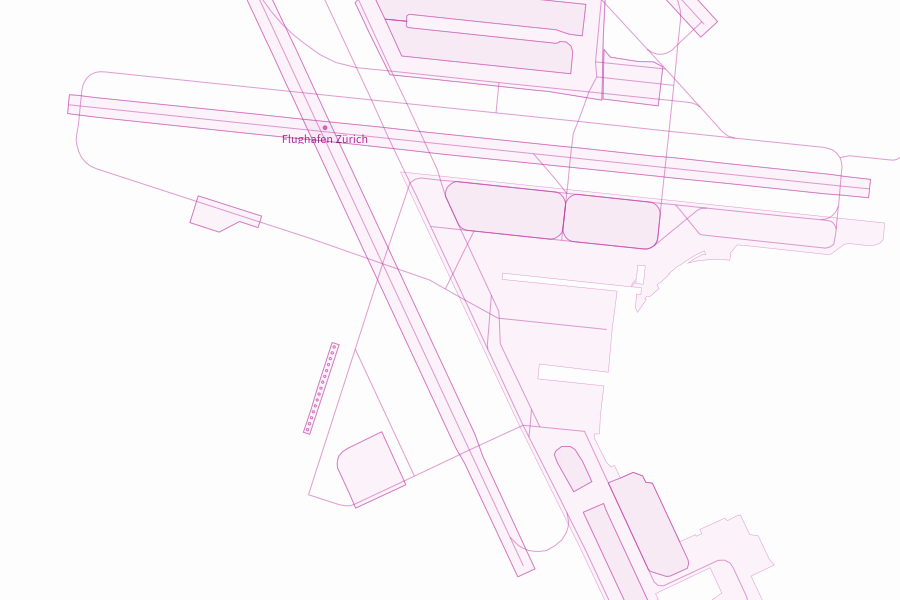
\includegraphics[width=1\textwidth]{images/schema/aeroway_example}
  \caption{Aerowaya and airport label layer of Zurich airport}
\end{figure}

%------------------------------------------------------
\subsection{Barriers}

The layer \textbf{barrier\_line} contains barriers that block a way or path. Common features are structural walls, fences or access controls like bicycle barriers and gates. Man made objects like piers or natural barriers like a cliff are contained as well in the \textbf{barrier\_line} layer. Despite the layer name barriers can not only be linestrings (e.g. walls) but polygons as well (e.g. piers). Barriers are only relevant at the highest zoom level 14.

\begin{figure}[H]
  \centering
  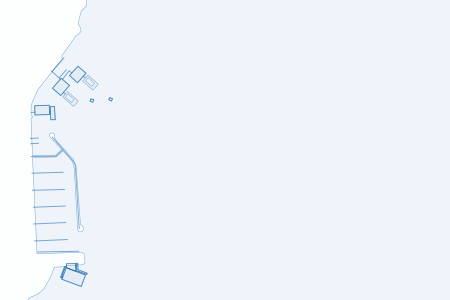
\includegraphics[width=1\textwidth]{images/schema/piers_example}
  \caption{Barrier line layer with piers at Lake Zurich}
\end{figure}

\begin{figure}[H]
  \centering
  \includegraphics[width=0.8\textwidth]{images/schema/barrier_line}
  \caption{Barrier layer Schema}
\end{figure}

%------------------------------------------------------
\subsection{Road and Road Labels}

Roads are one of the most essential features in maps. Roads are present across all zoom levels filtered by their importance. The \textbf{road} and \textbf{road\_label} layer query the data from the \textbf{road\_geometry} table where both polygons and linestrings are present.

The \textbf{road\_label} layer consists of linestrings that have a name assigned and are also encoded as linestrings in the vector tile. The actual client renderer takes care of putting the road label across the road linestring.

\begin{figure}[H]
  \centering
  \includegraphics[width=0.8\textwidth]{images/schema/road}
  \caption{Road layer schema}
\end{figure}

\begin{figure}[H]
  \centering
  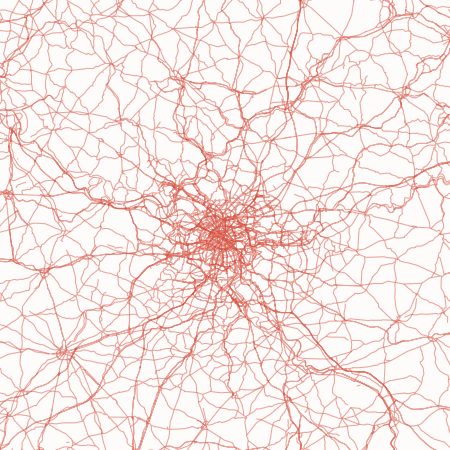
\includegraphics[width=1\textwidth]{images/schema/road_example}
  \caption{Road layer of France around Paris at zoom level 8}
\end{figure}

%------------------------------------------------------
\subsection{Water and Water Labels}



\begin{figure}[H]
  \centering
  \includegraphics[width=0.8\textwidth]{images/schema/water}
  \caption{Water layer schema}
\end{figure}

\begin{figure}[H]
  \centering
  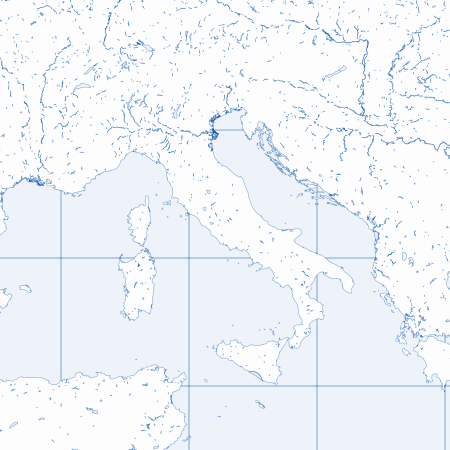
\includegraphics[width=1\textwidth]{images/schema/water_example}
  \caption{Tiled ocean and water bodies in Europe at zoom level 5}
\end{figure}

%------------------------------------------------------
\subsection{Buildings and Housenumber Labels}

\begin{figure}[H]
  \centering
  \includegraphics[width=0.8\textwidth]{images/schema/building}
  \caption{Building layer schema}
\end{figure}

\begin{figure}[H]
  \centering
  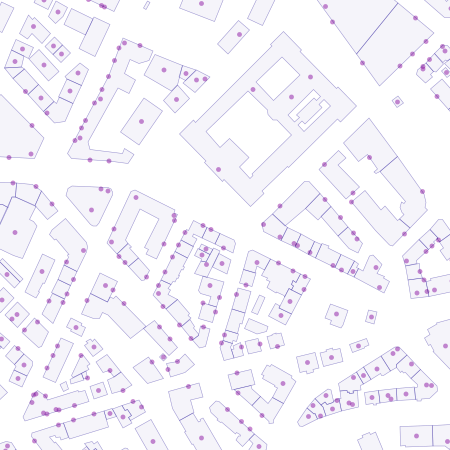
\includegraphics[width=1\textwidth]{images/schema/building_example}
  \caption{Buildings and house numbers at zoom level 17}
\end{figure}

%------------------------------------------------------
\subsection{Admin}

\begin{figure}[H]
  \centering
  \includegraphics[width=0.8\textwidth]{images/schema/admin}
  \caption{Admin layer schema}
\end{figure}

\begin{figure}[H]
  \centering
  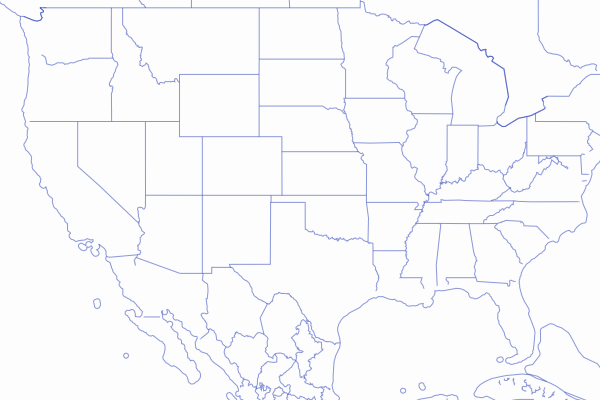
\includegraphics[width=1\textwidth]{images/schema/admin_example}
  \caption{Admin level 4 (states) in the US at zoom level 4}
\end{figure}

%------------------------------------------------------
\subsection{Landuse}

\begin{figure}[H]
  \centering
  \includegraphics[width=0.8\textwidth]{images/schema/landuse}
  \caption{Landuse layer schema}
\end{figure}

\begin{figure}[H]
  \centering
  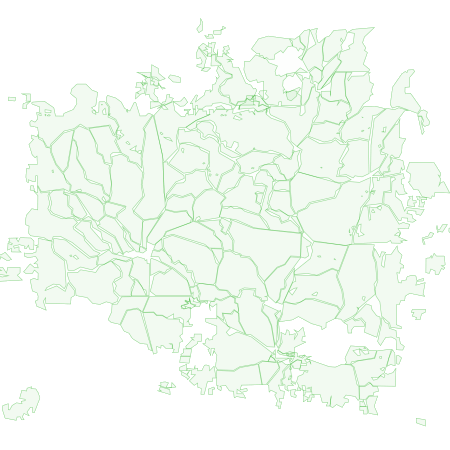
\includegraphics[width=1\textwidth]{images/schema/landuse_example}
  \caption{Landuse (wood) at zoom level 10}
\end{figure}